%%%%%%%%%%%%%%%%%%%%%%%%%%%%%%%%%%%%%%%%%%%%%%%%%%%%%%%%
%%%%%%%%%%%%%%%%%%%%%%%%%%%%%%%%%%%%%%%%%%%%%%%%%%%%%%%%
\newpage
\part{Backtracking}
\setcounter{section}{0}
%\begin{center}
%\huge{\textbf{Backtracking}} \\
%\end{center}

En general, el diseño de un algoritmo que resuelva un problema se puede considerar una tarea difícil. Una forma de facilitar esta tarea es recurrir a técnicas conocidas de diseño de algoritmos basados en esquemas muy generales que pueden adaptarse a un problema particular al detallar las partes generales del esquema. Muchos problemas pueden resolverse buscando una solución fácil y directa pero, a en otras oportunidades no resulta tan sencilla o simplemente es ineficiente. Un esquema de éstos se denomina backtracking el cual permite buscar todas las soluciones posibles de un problema incluyendo la óptima; pero no siempre resulta eficiente en tiempo y espacio.

Estudiaremos los aspectos de este esquema para el diseño de algoritmos.


%%%%%%%%%%%%%%%%%%%%%%%%%%%%%%%%%%%%%%%%%%%%%%%%%%%%%%%%
\section{Definiciones}

%Problemas que no se conoce su solución: ajedrez
El método del backtracking (también llamado búsqueda atrás o en retroceso) proporciona una manera sistemática de generar todas las posibles soluciones a un problema dentro de un espacio de búsqueda. Es posible definir el backtracking como un algoritmo general para encontrar un conjunto de soluciones a un problema computacional donde se va creando de forma incremental un conjunto de candidatos que formarán parte de una solución final. El algoritmo explora los elementos de un conjunto y selecciona/descarta subconjuntos de candidatos que pertenecen/no-pertenecen a la solución. Entonces dada una solución $s$:
\begin{enumerate}
\item Si $s$ es solución, se hace algo con ella (depende del problema)
\item Se construyen extensiones de $s$ y se invoca recursivamente al algoritmo con todas ellas
\end{enumerate}
La descripción natural del proceso se representa mediante un árbol de búsqueda en el que se muestra como cada tarea se descompone o se ramifica en subtareas. El árbol de búsqueda acaba en hojas donde se encuentran soluciones o donde se concluye que por esa rama no es posible encontrarla.


Este algoritmo debe ser aplicado a problemas donde existan elementos considerados ``candidatos parciales de la solución" para permitir realizar verificaciones rápidas si dichos candidatos pertenecen a la solución ó no. No resulta útil para conjuntos no ordenados, donde la exploración es total (explorar todos los candidatos). Entonces, el punto clave de los algoritmos de backtracking es: descartar/seleccionar rápidamente las soluciones inválidas/válidas. Esta es la diferencia principal con los algoritmos de fuerza bruta.

Es importante destacar que un algoritmo de fuerza bruta prueba todas las soluciones sin condición alguna, es decir, todas las posibles combinaciones. Por ejemplo, dado un número $b$ de bits obtener todos los valores posibles que se pueden representar.

En un problema, cuando se elimina la posibilidad de explorar todas las soluciones entonces estamos en presencia de un esquema de backtracking. Para ello, se requiere de una función llamada poda/acotación que permite identificar cuando una solución parcial no conduce a una solución al problema. Del mismo modo, se definen las restricciones asociadas a los problemas que pueden ser explícitas o implícitas. Se refiere a restricción explícita cuando restringe los posibles valores de las variables de forma individual, y explícitas cuando establece relaciones entre diferentes variables que forman una tupla candidato a solución.

%%%%%%%%%%%%%%%%%%%%%%%%%%%%%%%%%%%%%%%%%%%%%%%%%%%%%%%%
\section{Técnica de Backtracking}

Visto de otro modo, una solución debe expresarse como una n-tupla $(x_1, ..., x_n)$ donde los $x_i$ son elegidos de algún conjunto finito $S_i$. Usualmente el problema a resolver requiere encontrar un vector que maximice/minimice/satisfaga una función criterio $F(x_1,...,x_n)$. A veces, se busca todos los vectores que satisfagan $F$. 

En un algoritmo de backtracking con datos de entrada $P$ a resolver se pueden definir cinco funciones: aceptar, rechazar, primero, próximo y solución. Cada uno opera de la siguiente forma:
\begin{enumerate}
\item Inicio (P): Retorna el candidato parcial de la raíz del problema con datos $P$; sirviendo como inicialización
\item Aceptar (P, C): Retorna \textbf{true} si el candidato parcial $C$ es una solución de $P$, y falso en caso contrario
\item Rechazar (P, C): Retorna \textbf{true} si un candidato parcial $C$ no debería continuar su exploración ó búsqueda de más candidatos
\item Primero (P, C): Extrae el primer elemento/componente del candidato parcial $C$ llamado $s$
\item Próximo (P, s): Genera el próximo conjunto de candidatos posterior a $s$
\item Solución (P, c): El subconjunto $c \in P$ se considera solución.
\end{enumerate}

La llamada inicial del algoritmo se hace como $Backtrack (P, Inicio (P))$, donde Backtrack se puede escribir como:

\begin{lstlisting}[upquote=true, language=pseudo]
void Backtrack (Set P, C)
  if Rechazar (P, C) then Abortar ( ) end
  if Aceptar (P, C) then Solucion (P, C) end
  Set s = Primero (P, C)
  while not s.EsVacio() do
    Backtrack (P, s)
    s = Proximo (P, s)
  end
end

Backtrack (P, Inicio (P))
\end{lstlisting}

El backtracking es empleado en diversos ámbitos de la Computación tales como problemas de decisión (soluciones que satisfacen ciertas restricciones) y problemas de optimización (búsqueda de la mejor solución en base a una función objetivo). Cada solución es el resultado de una secuencia de decisiones. En algunos problemas de este tipo se conoce un criterio óptimo de selección en cada decisión (i.e. técnica voraz). En otros problemas se cumple el principio de optimalidad de Bellman y se puede aplicar la técnica de programación dinámica. Existen otros problemas en los que no hay más remedio que buscar en todo el espectro posible de soluciones.

Apliquemos el enfoque de backtracking para conseguir la permutación de una secuencia. Dado un String, se quiere imprimir todas las palabras producto de permutar el String. La permutación es una variación del orden o de disposición de los elementos de un conjunto. Por ejemplo, dada la palabra ``zen" las permutaciones posibles están formadas por las palabras ``zen", ``zne", ``ezn", ``enz", ``nez" y ``nze". Es importante destacar que en una permutación debe existir un orden para la construcción de la solución. De forma intuitiva, la solución se puede conseguir al fijar un carácter y mover los otros dos restantes y así para los tres caracteres de la palabra ``zen".

Algorítmicamente, dada la palabra inicial se consideran índices que indican ``desde cuál posición" se comienza a operar en la palabra y ``hasta cuál posición", es decir, los límites inferior y superior. En cada iteración del algoritmo, el límite inferior debe ir variando (ciclo) hasta el límite inferior. Debido a que cada iteración considera un límite inferior distinto, es posible crear un \textbf{estado} que representan el valor de las variables en un momento dado. Entonces, para cada estado se aplica la misma estrategia tal que siempre se \textbf{fijen} unas posiciones y otras se iteren.

La operación que permitirá el cambio de las letras de la palabra es el procedimiento $swap$. Este recibirá por referencia la palabra a modificar y cuáles son las posiciones a intercambiar. Ahora, para que un estado nuevo obtenga los valores correctos la palabra que ha sido intercambiada debe volver a su estado original (i.e. regresar los cambios). Por ello, se debe emplear nuevamente el procedimiento $swap$ luego de haber explorado nuevas soluciones.

\begin{figure}[htpb!]
  \begin{center}
    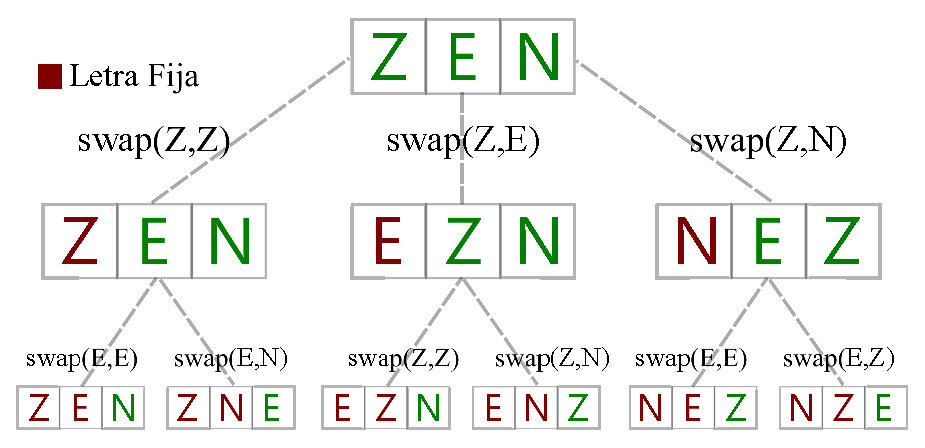
\includegraphics[width=0.7\textwidth]{images/backtracking.eps}
  \end{center}
  \caption{Esquema de ejecución de las permutaciones para la palabra ``Zen".}
  \label{fig:Ch2permutacion}
\end{figure}

El código asociado a la permutación de los caracteres de un String se puede escribir como:

\begin{lstlisting}[upquote=true, language=pseudo, numbers=left]
void Permute (String strText, Integer iIndex, iLength)
  if iIndex == iLength then
    Print (strText)
  else
    for Integer iJ = iIndex to iLength do
      swap (ref strText, iIndex, iJ)
      Permute (strText, iIndex + 1, iLength)
      swap (ref strText, iIndex, iJ) //backtrack
    end
end

String strText = "Zen"
Permute(strText, 1, 3)
\end{lstlisting}

La ejecución del algoritmo se muestra de forma gráfica en la Fig. \ref{fig:Ch2permutacion}. La idea detrás de la permutación es tener una posición fija de inicio de las iteraciones (línea 5) la cual debe ser empleada en cada invocación recursiva (línea 1). De este modo, desde esa posición en adelante se aplica el intercambio de la palabra inicial $iIndex$ con el índice de la iteración (línea 6). Luego, se invoca recursivamente la función pero ahora con un nuevo punto de partida (línea 7) y se ejecuta la misma idea. Posteriormente, el intercambio de letras (línea 6) no debe afectar el estado de ejecución de un estado, regresando el cambio realizado (línea 8). La solución se obtiene cuando el límite inferior alcanza al superior (línea 2), indicando que recorrió todas las posiciones de la palabra.


%%%%%%%%%%%%%%%%%%%%%%%%%%%%%%%%%%%%%%%%%%%%%%%%%%%%%%%%
\section{Clasificación}

Una solución de backtracking en cada iteración se encontrará en un cierto nivel $k$, con una solución parcial $C = (x_1, x_2, ..., x_k)$ (con $k \le n$). Entonces:
\begin{itemize}
\item Si puede añadirse un elemento $x_k + 1$ a la solución parcial se avanza al nivel $k + 1$
\item Si no se prueban otros valores válidos para $x_k$
\item Si no existe ningún valor que sea válido por probar, se retrocede al nivel anterior $k - 1$.
\end{itemize}
Así, se continua con este proceso hasta que la solución parcial sea una solución del problema o hasta que no queden más posibilidades por probar (en el caso de que no se encuentre ninguna solución o se busquen todas las soluciones del problema).

De esta forma, es posible clasificar un algoritmo de backtracking de acuerdo al tamaño del subconjunto $C$ solución:
\begin{itemize}
\item Una solución: Cuando el algoritmo encuentre una solución, su ejecución finaliza. Generalmente, en este enfoque el algoritmo se queda con la la primera solución que consigue.
\item Solución óptima: Cuando el algoritmo explora todos los subconjuntos de soluciones posibles y se queda con la óptima para el problema a resolver.
\item Todas las soluciones: El algoritmo colecta todos los subconjuntos encontrados en la exploración y forman parte de la solución (fuerza bruta).
\end{itemize}

Existen diversos algoritmos clásicos que se resuelven con algoritmos de backtracking: rompecabezas, laberintos, permutaciones, problemas de las 8-reinas, crucigramas, Sudoku, problema de la mochila, problema del agente viajero, entre otros. 

En backtracking, la generación de los estados solución o no en la exploración se generan en profundidad, es decir, seleccionando una opción y explorando todas las posibilidades a partir de ese punto. Por otro lado, existen enfoques donde para un estado se generan todos los posibles nuevos estados y antes de explorarlos, se verifican si conducen a una solución (branch \& bound).

%%%%%%%%%%%%%%%%%%%%%%%%%%%%%%%%%%%%%%%%%%%%%%%%%%%%%%%%
\section{Ejercicios}

La forma básica de resolver un problema aplicando backtracking es analizando los casos que son solución al problema y de qué forma se obtiene dicha solución. A continuación estudiaremos algunos casos.

\subsection{Suma Parcial}
Dado un conjunto de valores enteros se quiere encontrar todos los subconjuntos que entre sus elementos sumen un valor $k$. Por ejemplo, considerando el conjunto ${1, 2, 3}$ la idea es encontrar todos los subconjuntos que entre sus elementos sumen $k=4$. Para este ejemplo, se toma en cuenta el orden de los elementos, es decir, el subconjunto ${1, 3}$ será distinto de ${3, 1}$.

Entonces dividiendo el problema en elementos a considerar se tiene:
\begin{description}
\item [Alternativa]: Valores 1, 2 y 3
\item [Subtarea]: Suma acumulativa
\item [Solución]: Suma igual a 4
\end{description}

Para hacer un poco de abstracción, se asumen las funciones asociadas a un conjunto para agregar un valor y eliminar un elemento en éste, y la de imprimir sus valores de forma ordenada. El procedimiento que realiza es cálculo se puede escribir como:

\begin{lstlisting}[upquote=true, language=pseudo, numbers=left]
void FindSum(Array A of Integer [], Integer iN, iPartial, iTotal)
  if iPartial == iTotal then
    printSet()
  else
    for Integer iIndex = 1 to iN do
      if iPartial + A[iIndex] <= iTotal then
        addSet(A[iIndex])
        FindSum(A, iN, iPartial + A[iIndex], iTotal)
        removeSet()
      end
    end
  end
end

Integer A of Integer [] = {1,2,3}
Integer iTotal = 4
FindSum(A, 3, 0, iTotal)
\end{lstlisting}

La idea básica del algoritmo es buscar las sumas parciales de los elementos del arreglo obtenidas de sumar un elemento \textit{actual} con la suma acumulada (línea 9). Si dicha suma parcial es inferior o igual al total buscado entonces se agrega al conjunto solución (línea 10). Ahora, con una nueva suma parcial se invoca de forma recursiva a la función (línea 11) y de conseguir solución (línea 5) se imprime el conjunto. En caso contrario, la invocación hecha retorna al estado anterior y regresa/retorna el valor añadido al conjunto de sumas parciales (línea 12).

Para la invocación inicial del algoritmo (línea 19), se requiere el arreglo inicial $A$, el tamaño de éste, la suma parcial para el estado inicial (i.e. $iPartial = 0$) y el valor destino que se quiere alcanzar.

\subsection{n-Reinas}

El problema de las n-reinas consiste en colocar $n$ reinas en un tablero de ajedrez sin que se amenacen unas con otras. En Ciencias de la Computación, el problema con $n=8$ es un problema combinatorio clásico donde no puede haber dos reinas en una misma fila, columna o diagonal. Así, podemos definir los siguientes aspectos del problema para diseñar la solución:

\begin{description}
\item [Representación]: n-tuplas $x_1, x_2, x_3,..., x_k$ donde $x_i$ es la fila donde está la reina de la columna $i$
\item [Restricciones implícitas]: Las componentes $1, 2,..., n$
\item [Restricciones explícitas]: No puede haber 2 reinas en una misma fila/columna/diagonal
\item [Solución]: Empezar en la columna más abajo a la izquierda. \\
Si todas las reinas están colocadas entonces return true \\
Para cada posibilidad en las filas de una columna \\
    Si la reina puede ser colocada \\
    Escoger esta solución y llamar recursivamente con las otras reinas \\
    Si la recursión suceded entonces true \\
    Si la recursión ¡succed entonces probar en otra fila \\
Si todas las columnas han sido probadas, entonces return falso \\
\end{description}

El algoritmo se puede escribir como: 

\begin{lstlisting}[upquote=true, language=pseudo]
function Solve (Array aBoard of Integer[][], Integer iN, iCol) : Boolean
  if iCol > iN then
    return true
  end
  for Integer iRowToTry = 1 to iN do
    PlaceQueen(aBoard, iRowToTry, iCol)
    if Solve (aBoard, iN, iCol + 1) then
      return true
    end
    RemoveQueen(aBoard, iRowToTry, iCol)
  end
end
\end{lstlisting}

Los procedimientos $Place$ y $Remove$ se emplean para ubicar y quitar una reina de una posición respectivamente. Por otro lado, la función $Solve$ verifica que en el tablero estén colocadas las $iN$ reinas sin que se ataquen unas a otras.

Es interesante notar que con 8 reinas, el tamaño del espacio de soluciones es $8^8$, es decir, $2^{24} \sim 16M$. Sin embargo, dado que las soluciones posibles son todas las permutaciones del conjunto ${1,2,3,4,5,6,7,8}$, el espacio de soluciones se reduce a de $8^8$ tuplas a $8! = 40.320$. Para explorar un caso más simple, en la Fig. \ref{fig:Ch2queen} se observan los estados generados en la ejecución cuando $n=4$ reinas en el tablero.

\begin{figure}[htpb!]
  \begin{center}
    \includegraphics[width=0.7\textwidth]{images/reinas4.jpg}
  \end{center}
  \caption{Estados generados para $n=4$ en el problema de las n-reinas.}
  \label{fig:Ch2queen}
\end{figure}

\subsection{Sudoku}

El Sudoku es un juego matemático que consiste en rellenar una cuadrícula de $9 \times 9$ celdas (81 casillas) dividida en subcuadrículas de $3 \times 3$ con las cifras del 1 al 9 partiendo de algunos números ya dispuestos en algunas de las celdas. Entonces, los números no se deben repetir en una misma fila, columna o subcuadrícula. Cuando existen al menos 17 valores en la cuadrícula entonces la solución es única, en caso contrario, puede tener varias formas de conseguir una solución.

El algoritmo para su resolución se plantea como un backtracking donde se van colocando números válidos del $[1..9]$ hasta que en la cuadrícula no se puedan colocar nuevos números. Así, en cada invocación se busca la casilla disponible y se intenta colocar un número. Dicho número debe cumplir las condiciones de ser único en una fila, columna y subcuadrícula, y si es posible se procede a invocar nuevamente a la misma función con el tablero modificado. En caso de que dicho número colocado en una posición no forme parte de una solución parcial, entonces se libera dicha posición para ser empleado en otra invocación.

Es posible escribir el algoritmo de la siguiente forma:

\begin{lstlisting}[upquote=true, language=pseudo, numbers=left]
function SolveSudoku(Array aGrid of Integer [][], Integer iN) : Boolean
  Integer iRow, iCol
  // If there is no unassigned location, we are done
  if not FindUnassignedLocation(aGrid, ref iRow, ref iCol) then
    return true // success!
  end
  for Integer iNum = 1 to 9 do    // consider digits 1 to 9
    if isSafe(aGrid, iRow, iCol, iNum) then
      aGrid[iRow][iCol] = iNum    // make tentative assignment
      if SolveSudoku(aGrid, iN) then
        return true
      end
      aGrid[iRow][iCol] = UNASSIGNED // failure, unmake & try again
    end
  end
  return false
end

Integer iN = 9
Array aGrid of Integer [1..iN][1..iN]
FillWithNumbersAndUnassigned(ref aGrid, iN)
if SolveSudoku(aGrid, iN) then
  PrintGrid(aGrid, iN)
else
  Print("No solution for you")
end
\end{lstlisting}

En un inicio, el tablero se inicializa con valores numéricos válidos y casillas libres o sin asignar (línea 20). La función de solución del backtracking se determina cuando no se pueda encontrar casillas libres para colocar un nuevo número (línea 4). En caso de existir una casilla libre se itera sobre el rango $[1..9]$, y de ser posible ubicar un número se coloca en la dicha casilla disponible (línea 9) y se repite el proceso de forma recursiva. Cuando la opción de colocar el número no sea adecuada, se desmarca dicha casilla asignándole el valor $UNASSIGNED$ y sea libre para otro estado del algoritmo (línea 13).

%%%%%%%%%%%%%%%%%%%%%%%%%%%%%%%%%%%%%%%%%%%%%%%%%%%%%%%%
\section{Algoritmos}

Muchos problemas pueden ser resueltos empleando el esquema de backtracking, entre ellos el problema del agente viajero (\textit{travelling salesman problem}), cápsula convexa (\textit{convex hull}), resolución de tableros y laberintos, coloración de grafos y regiones, entre muchos otros.

\subsection{Laberinto}

El concepto de laberinto básico es dada una posición inicial encontrar la salida en otra posición. Para simplificar un poco, dada una matriz de tamaño $Size_x \times Size_y$ que representa al laberinto, se desea encontrar el conjunto de movimientos a realizar para encontrar la salida en la posición $Size_x$ y $Size_y$, empezando desde la posición $(1,1)$. Se asume que el laberinto puede tener posiciones libres (por donde se puede pasar) o bloqueadas (paredes).

\begin{lstlisting}[upquote=true, language=pseudo]
class Back
private:
	Const Integer FREE = 0
	Const Integer VISITED = 1
	Const Integer WALL = 2
	Array m_aMoveX of Integer [] = {-1, +1, 0, 0}
	Array m_aMoveY of Integer [] = {0, 0, -1, +1}
	Array m_aTable of Integer [][]
	Integer m_iSizeX, m_iSizeY
	Set m_sSolution
	void setRandomWalls(Integer iSizeX, iSizeY)	//add some walls
	function isValid(Integer iPosX, iPosY) : Boolean
		return iPosX >= 1 and iPosX <= iSizeX and iPosY >= 1 and iPosY <= iSizeY and m_aTable[iPosX][iPosY] == FREE
	end
public:
	Constructor Back(Integer iSizeX, iSizeY)
		m_iSizeX = iSizeX
		m_iSizeY = iSizeY
		m_aTable = new Integer[1..m_iSizeX][1..m_iSizeY]
		m_sSolution = {}
		for Integer iY to m_iSizeY do
			for Integer iX to m_iSizeX do
				m_aTable[iX][iY] = FREE
			end
		end
		setRandomWalls(iSizeX, iSizeY)
	end

	void Labyrinth (Integer iStepX, iStepY)
		Boolean bSolution = false
		if iStepX == iSizeX and iStepY == iSizeY then
			bSolution = true
			PrintSet()
		end
		m_aTable[iStepX][iStepY] = VISITED
		Integer iDirection = 1
		while not bSolution and iDirection <= 4 do
			if isValid(iStepX + m_aMoveX[iDirection], iStepY + m_aMoveY[iDirection]) then
				addSet(iStepX + m_aMoveX[iDirection], iStepY + m_aMoveY[iDirection])
				Labyrinth (iStepX + m_aMoveX[iDirection], iStepY + m_aMoveY[iDirection])
				removeSet(iStepX + m_aMoveX[iDirection], iStepY + m_aMoveY[iDirection])
			end
			iDirection = iDirection + 1
		end
	end
end
\end{lstlisting}

%metro 391 bs pared 
%piso 570 bs
%900 bs

%cierran a las 5pm, abren a las 9am

\subsection{Problema de la Mochila}

El problema de la mochila o \textit{Knapsack} consiste en llenar una mochila con una serie de objetos asociados a una serie de pesos con un valor asociado. Es decir, se dispone de $iN$ tipos de objetos y que no hay un número limitado de cada tipo de objeto (si fuera limitado no cambia mucho el problema). Cada tipo $i$ de objeto tiene un peso $aWeight[i]$ positivo y un valor $aValue[i]$ positivo asociados. 

La mochila tiene una capacidad de peso igual a $iCapacity$. Se trata de llenar la mochila de tal manera que se maximice el valor de los objetos incluidos pero respetando al mismo tiempo la restricción de capacidad. 

\begin{lstlisting}[upquote=true, language=pseudo]
Array aWeight of Integer [] = {2, 3, 4, 5}
Array aValue of Integer [] = {3, 5, 6, 10}
Integer iN = 4

void Knapsack (Integer iStart, iCapacity, iSolution, ref iOptimal)
  for Integer iK = iStart to iN do
    if aWeight[iK] <= iCapacity then
      Knapsack (iK, iCapacity - aWeight[k], iSolution + aValue[iK], iOptimal)
      if iSolution + aValue[k] > iOptimal then
        iOptimal = iSolution + aValue[k]
      end
    end
  end
end

Integer iCapacity = 8, iOptimal = 0
Knapsack (1, iCapacity, 0, ref iOptimal)
Print (iOptimal)
\end{lstlisting}

%%%%%%%%%%%%%%%%%%%%%%%%%%%%%%%%%%%%%%%%%%%%%%%%%%%%%%%%
\section{Ideas Finales}

\begin{itemize}
\item El backtracking es un método sistemático que realiza una búsqueda exhaustiva de las soluciones, pero esta búsqueda no es caótica, sino organizada
\item Esta permite obtener una o todas las soluciones factibles o bien la solución óptima entre todas las factibles
\item La técnica del backtracking se puede implementar como una versión iterativa empleando estructuras de datos para almacenar los estados candidatos a solución
\item El costo de aplicar una solución de backtracking es proporcional al número de estados que se generan en las invocaciones recursivas
\end{itemize}

%%%%%%%%%%%%%%%%%%%%%%%%%%%%%%%%%%%%%%%%%%%%%%%%%%%%%%%%
\section{Problemas}
\begin{figure}[htpb!]
  \begin{center}
    \includegraphics[width=0.3\textwidth]{images/rushhour.jpg}
  \end{center}
  \caption{Un estado del juego \textit{Rush Hour}.}
  \label{fig:Ch2rush}
\end{figure}
\begin{enumerate}
\item Dado un número entero $n$ se desea obtener todas las posibles formas de expresarlo como sumas de los enteros $1...n$, permitiendo que el mismo sumando aparezca varias veces. Se considerarán iguales (y por lo tanto sólo se debe escribir una de ellas) aquellas soluciones que contengan los mismos sumandos pero ordenados de otra manera. Por ejemplo, si $n = 4$, se deberían escribir las soluciones $4=1+1+1+1$, $4=2+1+2$, $4=2+2$, $4=3+1$, $4=4$. Crear un algoritmo que resuelva el problema. No es relevante el orden en que aparecen las soluciones ni el orden de los sumandos dentro de cada solución
\item En criptografía, un ataque de fuerza bruta es la forma de recuperar una clave probando todas las combinaciones posibles hasta encontrar el acceso a un sistema. Implemente una función $Hacking$ que obtenga la clave de un usuario conociendo que está tiene un mínimo de 5 y máximo 12 caracteres alfanuméricos
\item En un colegio, se tienen $k$ botellas de plástico que van a ser reusadas. Las botellas tienen distinto largo $t_i$, el objetivo es juntar/pegar las botellas unas con otras por sus extremos para construir árboles de navidad, aviones, barcos, edificios, y otras estructuras para la educación. Cada estructura es de largo $L$ y debe emplear la mayor cantidad de botellas para ser reusadas, construya el algoritmo que resuelva el algoritmo para el problema
\item Dado un conjunto de canciones $c_1, c_2, ..., c_k$ que ocupan $m_1, m_2, ..., m_k$ espacio respectivamente, se desea construir una solución que permita maximizar el número de canciones almacenadas en un dispositivo externo de capacidad $M$
\item Proponga un esquema que resuelva el conocido cubo de Rubik. ¿Cuáles alternativas se deben considerar en su resolución?
\item \textit{Rush Hour} es un rompecabezas de bloque con deslizamientos creado en 1970. En su versión original, consiste de un tablero de $6 \times 6$ donde se ubican una serie de carros y camiones (los carros ocupan 2 posiciones y los camiones 3 posiciones). La idea del juego es sacar todos los autos por la salida deslizando los autos colocados en el tablero. Construya un algoritmo que resuelva el problema en el menor número de deslizamientos en el tablero.
\end{enumerate}

